\documentclass{exam}
\usepackage{../../commonheader}
\lstset{language=Scheme}

%%% CHANGE THESE %%%%%%%%%%%%%%%%%%%%%%%%%%%%%%%%%%%%%%%%%%%%%%%%%%%%%%%%%%%%%%
\discnumber{8}
\title{\textsc{Streams, Iterators, & Generators}}
\date{April 4 to April 9, 2016}
%%%%%%%%%%%%%%%%%%%%%%%%%%%%%%%%%%%%%%%%%%%%%%%%%%%%%%%%%%%%%%%%%%%%%%%%%%%%%%%

\begin{document}
\maketitle
\rule{\textwidth}{0.15em}
\fontsize{12}{15}\selectfont

%%% INCLUDE TOPICS HERE %%%%%%%%%%%%%%%%%%%%%%%%%%%%%%%%%%%%%%%%%%%%%%%%%%%%%%%


%%% Question %%%

\section{Streams}
\begin{questions}
\begin{blocksection}
\question What’s the advantage of using a stream over a linked list?
\begin{solution}[0.2in] 
Lazy evaluation. We only evaluate up to what we need.
\end{solution}

\quesiton What’s the maximum size of a stream?
\begin{solution}[0.2in]
Infinity
\end{solution}

\question What’s stored in first and rest? What are their types? 
\begin{solution}[0.2in]
First is a value, rest is another stream (either a method to calculate it, or an already calculated stream). In the case of Scheme, this is called a promise.
\end{solution}

\question When is the next element actually calculated?
\begin{solution}[.2in]
Only when it's requested (and hasn't already been calculated)
\end{solution}
\end{blocksection}

\section{What Would Scheme Print?}
\begin{blocksection}
\question For each of the following lines of code, write what scheme would output.

\begin{lstlisting}
scm> (define x 1)
\end{lstlisting}
\begin{solution}[.25in]
\texttt{x}
\end{solution}

\begin{lstlisting}
scm> (if 2 3 4)
\end{lstlisting}
\begin{solution}[.25in]
\texttt{3}
\end{solution}

\begin{lstlisting}
scm> (delay (+ x 1))
\end{lstlisting}
\begin{solution}[.25in]
\texttt{#[promise]}
\end{solution}

\begin{lstlisting}
scm> (define (foo x) (+ x 10))
\end{lstlisting}
\begin{solution}[.25in]
\texttt{foo}
\end{solution}

\begin{lstlisting}
scm> (define bar (cons-stream (foo 1) (cons-stream (foo 2) bar)))
\end{lstlisting}
\begin{solution}[.25in]
\texttt{bar}
\end{solution}

\begin{lstlisting}
scm> (car bar)
\end{lstlisting}
\begin{solution}[.25in]
\texttt{11}
\end{solution}
\end{blocksection}

\begin{blocksection}
\begin{lstlisting}
scm> (cdr bar)
\end{lstlisting}
\begin{solution}[.25in]
\texttt{#[promise]}
\end{solution}

\begin{lstlisting}
scm> (define (foo x) (+ x 1))
\end{lstlisting}
\begin{solution}[.25in]
\texttt{foo}
\end{solution}

\begin{lstlisting}
scm> (cdr-stream bar)
\end{lstlisting}
\begin{solution}[.25in]
\texttt{(3 . #[promise])}
\end{solution}

\begin{lstlisting}
scm> (define (foo x) (+ x 5))
\end{lstlisting}
\begin{solution}[.25in]
\texttt{foo}
\end{solution}

\begin{lstlisting}
scm> (car bar)
\end{lstlisting}
\begin{solution}[.25in]
\texttt{11}
\end{solution}

\begin{lstlisting}
scm> (cdr-stream bar)
\end{lstlisting}
\begin{solution}[.25in]
\texttt{(3 . #[promise])}
\end{solution}

\begin{lstlisting}
scm> (define (foo x) (+ x 5))
\end{lstlisting}
\begin{solution}[.25in]
\texttt{foo}
\end{solution}

\begin{lstlisting}
scm> (car bar)
\end{lstlisting}
\begin{solution}[.25in]
\texttt{11}
\end{solution}

\begin{lstlisting}
scm> (cdr-stream bar)
\end{lstlisting}
\begin{solution}[.25in]
\texttt{(3 . #[promise])}
\end{solution}
\end{blocksection}

\section{Code Writing Questions for Streams}

%%% Question %%%
\begin{blocksection}
\question Write out \texttt{double_naturals}, which is a stream that evaluates to the sequence 1, 1, 2, 2, 3, 3, etc.
\begin{lstlisting}
(define (double_naturals)
    (double_naturals_helper 1 0)
)

(define (double_naturals_helper first flag)




)
\end{lstlisting}

\begin{solution}[1in]
\begin{lstlisting}
(define (double_naturals_helper first flag)
    (if (= 1 flag)
        (cons-stream first (double_naturals_helper (+ 1 first) 0))
        (cons-stream first (double_naturals_helper first 1))
    )
)

;Alternative Solutions
(define (double_naturals_helper first flag)
    (cons-stream first (double_naturals_helper (+ flag first) (- 1 flag)))
)
\end{lstlisting}
\end{solution}

\question Write out \texttt{interleave}, which returns a stream that alternates between the values in stream1 and stream2. Assume that the streams are infinitely long.
\begin{lstlisting}
(define (double_naturals)
    (double_naturals_helper 1 0)
)

(define (double_naturals_helper first flag)




)
\end{lstlisting}

\begin{solution}[1in]
\begin{lstlisting}
(define (double_naturals_helper first flag)
    (if (= 1 flag)
        (cons-stream first (double_naturals_helper (+ 1 first) 0))
        (cons-stream first (double_naturals_helper first 1))
    )
)

;Alternative Solutions
(define (double_naturals_helper first flag)
    (cons-stream first (double_naturals_helper (+ flag first) (- 1 flag)))
)
\end{lstlisting}
\end{solution}
\end{blocksection}

%%% Question %%%
\section{Scheme Lists}
\begin{blocksection}
\begin{nonsol}
Scheme has linked lists built in. You can make the following analogy:
\begin{center}
\begin{tabular}{ |l|l| }
\hline
 \texttt{Link(1, Link.empty)} & \texttt{(cons 1 nil)} \\
 \texttt{a = Link(1, Link(2, Link.empty))} & \texttt{(define a (cons 1 (cons 2 nil)))}  \\
 \texttt{a.first} & \texttt{(car a)} \\
 \texttt{a.rest} & \texttt{(cdr a)} \\
 \hline
\end{tabular}
\end{center}
However, \textbf{Scheme \texttt{cons} is more powerful}, as it allows its second argument to not be a list. Try the following out in the interpreter. Draw box and pointers when appropriate. Ask your mentor if you're unsure what's going on. You aren't expected to understand this completely on your own.
\question What will Scheme output? Draw box-and-pointer diagrams to help determine this.
\end{nonsol}

\begin{lstlisting}
scm> (cons 1 2)
\end{lstlisting}
\begin{solution}[0.25in]
\texttt{(1 . 2)}
\begin{center}
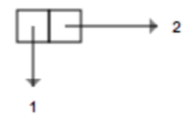
\includegraphics[scale=0.7]{9a}
\end{center}
\end{solution}

\begin{lstlisting}
scm> (cons 1 (cons 2 nil))
\end{lstlisting}
\begin{solution}[0.25in]
\texttt{(1 2)}
\begin{center}
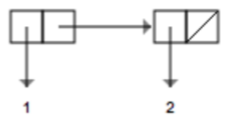
\includegraphics[scale=0.7]{9b}
\end{center}
\end{solution}

\begin{lstlisting}
scm> (cons 1 '(2 3 4 5))
\end{lstlisting}
\begin{solution}[0.25in]
\texttt{(1 2 3 4 5)}
\begin{center}
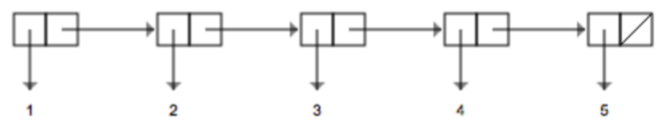
\includegraphics[scale=0.7]{9c}
\end{center}
\end{solution}

\begin{lstlisting}
scm> (cons 1 '(2 (cons 3 4))
\end{lstlisting}
\begin{solution}[0.25in]
\texttt{(1 2 (cons 3 4))}
\begin{center}
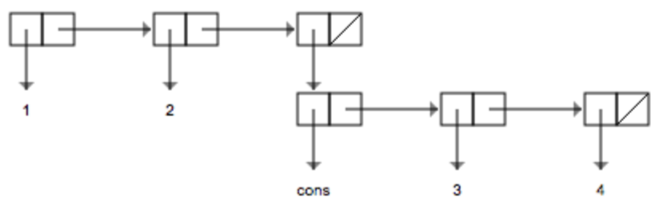
\includegraphics[scale=0.7]{9d}
\end{center}
\end{solution}

\begin{lstlisting}
scm> (cons 1 (2 (cons 3 4)))
\end{lstlisting}
\begin{solution}[.25in]
\begin{lstlisting}
eval: bad function in : (2 (cons 3 4))
\end{lstlisting}
\end{solution}
\end{blocksection}

\begin{blocksection}
\begin{lstlisting}
scm> (define a '(1 2 . 3))
\end{lstlisting}
\begin{solution}[.25in]
\begin{lstlisting}
a
\end{lstlisting}
\end{solution}

\begin{lstlisting}
scm> a
\end{lstlisting}
\begin{solution}[.25in]
\begin{lstlisting}
(1 2 . 3)
\end{lstlisting}
\end{solution}

\begin{lstlisting}
scm> (car a)
\end{lstlisting}
\begin{solution}[.25in]
\begin{lstlisting}
1
\end{lstlisting}
\end{solution}

\begin{lstlisting}
scm> (cdr a)
\end{lstlisting}
\begin{solution}[.25in]
\begin{lstlisting}
(2 . 3)
\end{lstlisting}
\end{solution}

\begin{lstlisting}
scm> (cadr a)
\end{lstlisting}
\begin{solution}[.25in]
\begin{lstlisting}
2
\end{lstlisting}
\end{solution}

How can we get the 3 out of a?
\begin{solution}[.25in]
\begin{lstlisting}
(cddr a)
\end{lstlisting}
\end{solution}
\end{blocksection}

\section{More Code Writing in Scheme}

%%% Question %%%
\begin{blocksection}
\question Define \texttt{well-formed}, which determines whether \texttt{lst} is a well-formed list or not. Assume that \texttt{lst} only contains numbers.

\begin{lstlisting}
; Doctests
> (well-formed '())
true
> (well-formed '(1 2 3))
true
; List doesn't end in nil
> (well-formed (cons 1 2))
false
; Nested lists are ok
> (well-formed (cons (cons 1 2) nil))
true
\end{lstlisting}

\begin{solution}[0.75in]
\begin{lstlisting}
; well-formed with a nested if statement
(define (well-formed lst)
    (if (null? lst)
        #t
        (if (number? lst)
            #f
            (well-formed (cdr lst)))))

; well-form with a cond statement
(define (well-formed lst)
    (cond ((null? lst) #t)
        ((number? lst) #f)
        (else (well-formed (cdr lst)))))
\end{lstlisting}
\end{solution}
\end{blocksection}

%%% Question %%%
\begin{blocksection}
\question Define \texttt{is-prefix}, which takes in a list \texttt{p} and a list \texttt{lst} and determines if \texttt{p} is a prefix of \texttt{lst}.

\begin{lstlisting}
; Doctests:
> (is-prefix '() '())
true
> (is-prefix '() '(1 2))
true
> (is-prefix '(1) '(1 2))
true
> (is-prefix '(2) '(1 2))
false
; Note here p is longer than lst
> (is-prefix '(1 2) '(1))
false
\end{lstlisting}

\begin{solution}[0.5in]
\begin{lstlisting}
; Same as below, but with cond
(define (is-prefix p lst)
    (cond ((null? p) #t)
        ((null? lst) #f)
        (else (and (= (car p) (car lst))
            (is-prefix (cdr p) (cdr lst))))))

; Solution that checks if lst is null for the last doctest
(define (is-prefix p lst)
    (if (null? p)
        #t
        (if (null? lst)
            #f
            (and
                (= (car p) (car lst))
                (is-prefix (cdr p) (cdr lst))))))
\end{lstlisting}
\end{solution}
\end{blocksection}

\end{questions}

%%%%%%%%%%%%%%%%%%%%%%%%%%%%%%%%%%%%%%%%%%%%%%%%%%%%%%%%%%%%%%%%%%%%%%%%%%%%%%%

\end{document}
